\documentclass[logo]{pbml}
\usepackage{latexsym}
\usepackage{graphicx}
\usepackage{amsmath}
\usepackage{wrapfig}
\usepackage{url}

\title{Visualizing Data Structures in Parsing-based Machine Translation}
%\subtitle{}

\author{firstname=Jonathan, surname=Weese,
       address={Department of Computer Science and Center for Language and Speech Processing \\
Johns Hopkins University \\
Baltimore, MD 21218, USA \\
{\tt jonny@cs.jhu.edu}}}
\author{firstname=Chris, surname=Callison-Burch, 
       address={Department of Computer Science and Center for Language and Speech Processing \\
Johns Hopkins University \\
Baltimore, MD 21218, USA \\
{\tt ccb@cs.jhu.edu}}}

\shorttitle{Visualizing Machine Translation}
\shortauthor{J. Weese, C. Callison-Burch}

\begin{document}
\maketitle
\begin{abstract}

As machine translation (MT) systems grow more complex and incorporate more
linguistic knowledge, it becomes more difficult to evaluate independent
pieces of the MT pipeline.
Being able to inspect many of the intermediate data structures used during
MT decoding allows a more fine-grained evaluation of MT performance, helping
to determine which parts of the current process are effective and which are
not.
In this article, we present an overview of the visualization tools that are
currently distributed with the Joshua \cite{Joshua-WMT} MT decoder.
We explain their use and present an example of how visually 
inspecting the decoder's data structures has led to useful improvements in
the MT model.

\end{abstract}

%{\sc
%Here are some citations to work into the text
%\begin{itemize}
%\item Syntax Augmented Machine Translation \cite{samt2006,zoll:08,Venugopal2009}
%\item Hiero \cite{Chiang2005,Chiang2007}
%\item Hypergraph citations \cite{billott-lang:1989:ACL,Klein2001}
%\end{itemize}
%}

\section{Introduction}





The Joshua machine translation decoder uses a 
formalism known as synchronous context-free grammars (SCFGs) \cite{Chiang2006}.
A probabilistic SCFG consists of a set of source-language terminal symbols, a set of target-language terminal symbols, a set of nonterminals
that is shared between both languages, and set of production rules of the
form
$$X \to \langle \gamma,\alpha,\sim,w \rangle$$
where $X$ is a nonterminal symbol, $\gamma$ is a (possibly mixed) sequence of
nonterminals and source terminals, $\alpha$ is a (again possibly mixed)
sequence of nonterminals and target-language terminals, $\sim$ is a one-to-one
correspondence between the nonterminals of $\gamma$ and $\alpha$, and $w$ is
a weight for the production rule.
%where $X \in N, \gamma \in [N \cup T_S]*$ is a (possibly mixed) sequence of
%nonterminals and source terminals, $\alpha \in [N \cup T_T]*$ is a 
%(again possibly mixed) sequence of nonterminals and target-language terminals,
% and $\sim$ is a one-to-one correspondence between the nonterminals of $\gamma$ and $\alpha$.
%$w$ is a weight for the production rule.

Using an SCFG to parse the input sentence automatically creates a corresponding target-language sentence.
We take the generated sentence as a candidate translation for the
input sentence. The sequence of rules used to generate $t_1^m$ is
called a {\it derivation}. The derivation encodes synchronous parse trees on
the source and target sides.

%As an example, consider the grammar with production rules
%\begin{align*}
%\textrm{PP} & \to \langle \textrm{ PREP}_1 \textrm{ NP}_2, \textrm{ PREP}_1 \textrm{ NP}_2 \rangle \\
%\textrm{NP} & \to \langle \textrm{ DET}_1 \textrm{ NN}_2, \textrm{ DET}_1 \textrm{ NN}_2 \rangle \\
%\textrm{PREP} & \to \langle \textit{ sur}, \textit{ on } \rangle \\
%\textrm{DET} & \to \langle \textit{ la}, \textit{ the } \rangle \\
%\textrm{NN} & \to \langle \textit{ lune}, \textit{ moon } \rangle
%\end{align*}
%The subscripts on nonterminals on the right hand side of a production rule
%represent the one-to-one correspondence $\sim$. For example, in the first rule,
%the PREP nonterminals are aligned, and the NP nonterminals are aligned.
%Figure \ref{toy-tree-figure} shows a parse tree for the French phrase
%``{\it sur la lune}'' and its automatically-generated candidate translation
%``on the moon.''

%In practice these grammars are automatically extracted and weighted using
%a bilingual parallel corpus. There are typically thousands of rules that may
%apply for a given input sentence and thousands of possible derivations and
%candidate translations.

Since we are parsing the input sentence with a probabilistic grammar, we can
generate many possible candidate parses for a particular sentence. These parses
may share a lot of structure --- for example, two different parse trees may
contain subtrees that are identical. 
As part of the search procdeure, the Joshua system compactly stores 
these structure-sharing
trees as a {\em hypergraph} or {\em packed forest} where identical subtrees
from many parses are represented by a single copy.
Structure-sharing hypergraphs are commonly used to represent the result of
parsing a sentence with a probabilistic CFG \cite{billott-lang:1989:ACL,Klein2001}.
So it is natural that Joshua's
SCFG-based model should use this data structure.

\begin{figure}
\begin{center}
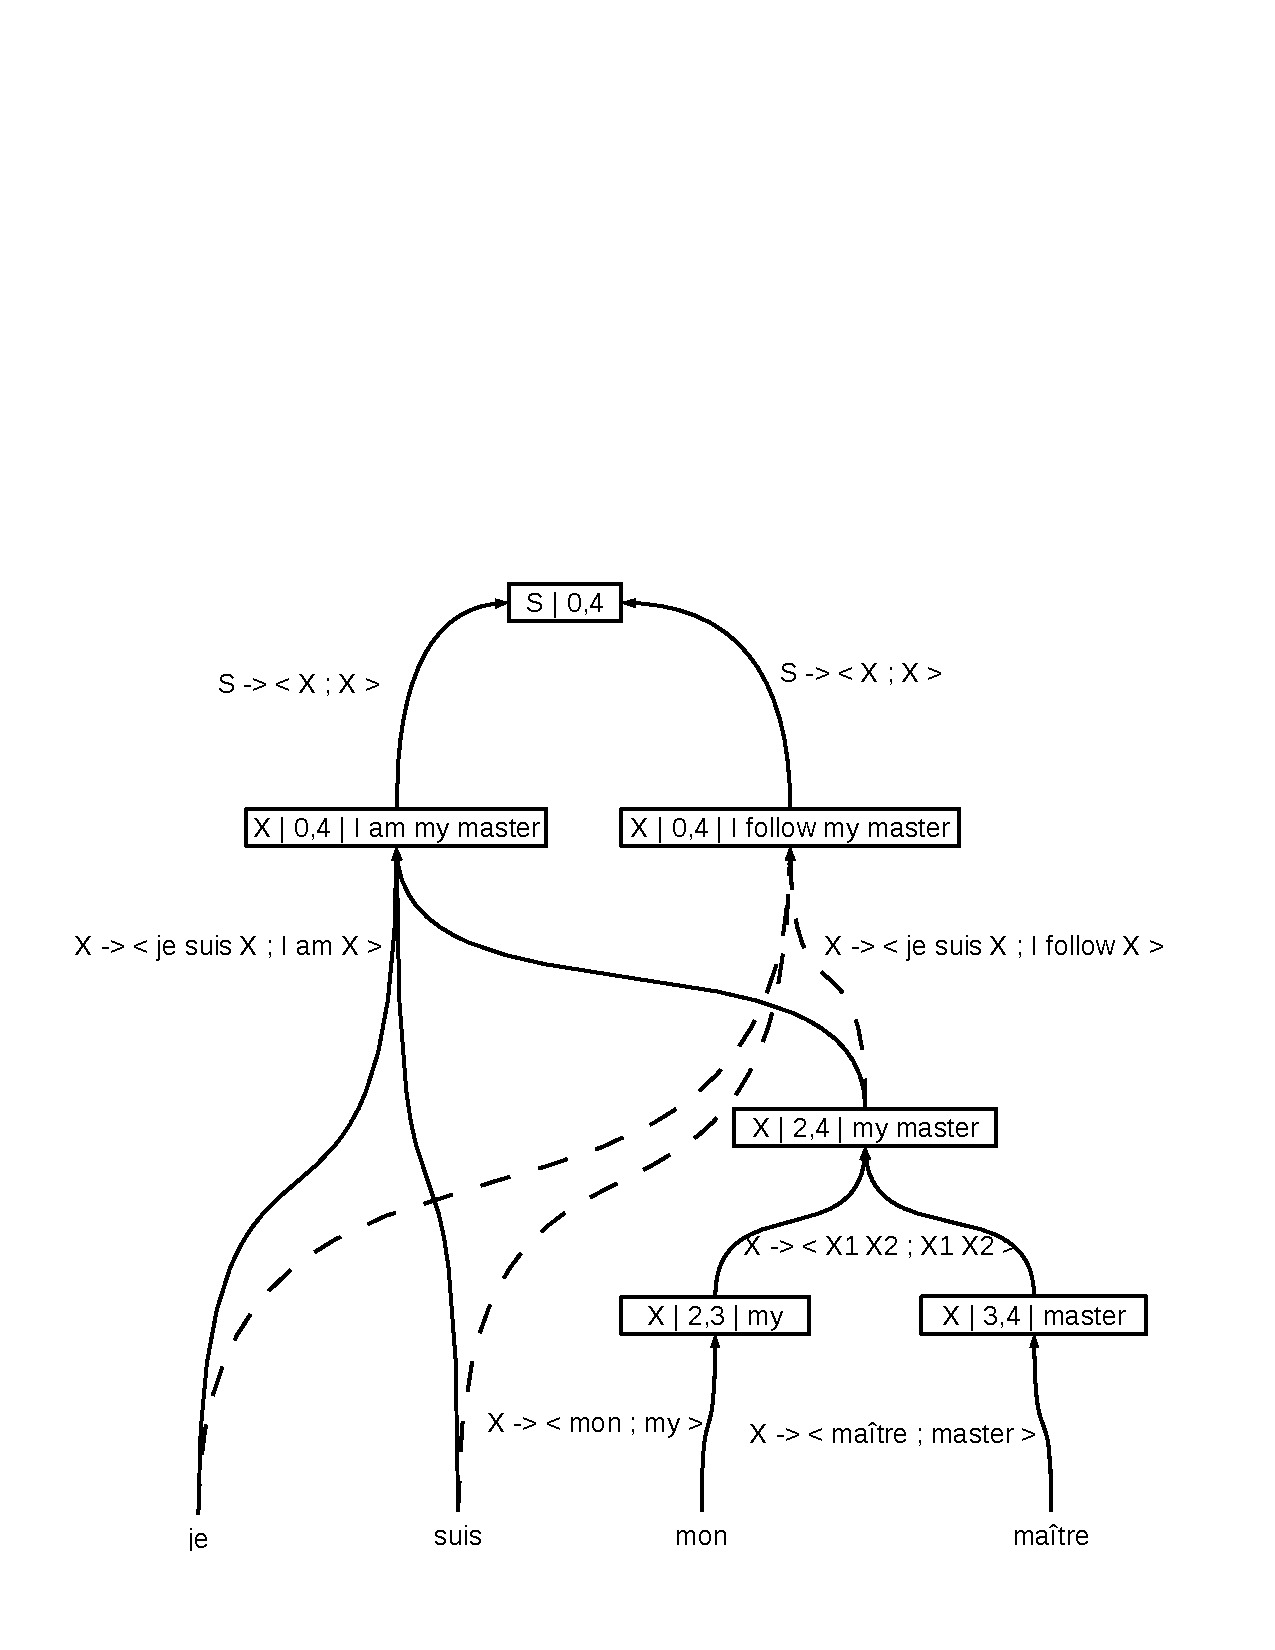
\includegraphics[height=3in]{images/hypergraph-example}
\end{center}
\caption{A hypergraph showing two candidate translations of {\it Je suis mon
ma\^{i}tre}.}
\label{hypergraph-example-figure}
\end{figure}


%\begin{wrapfigure}{r}{.66\linewidth}
%\begin{center}
%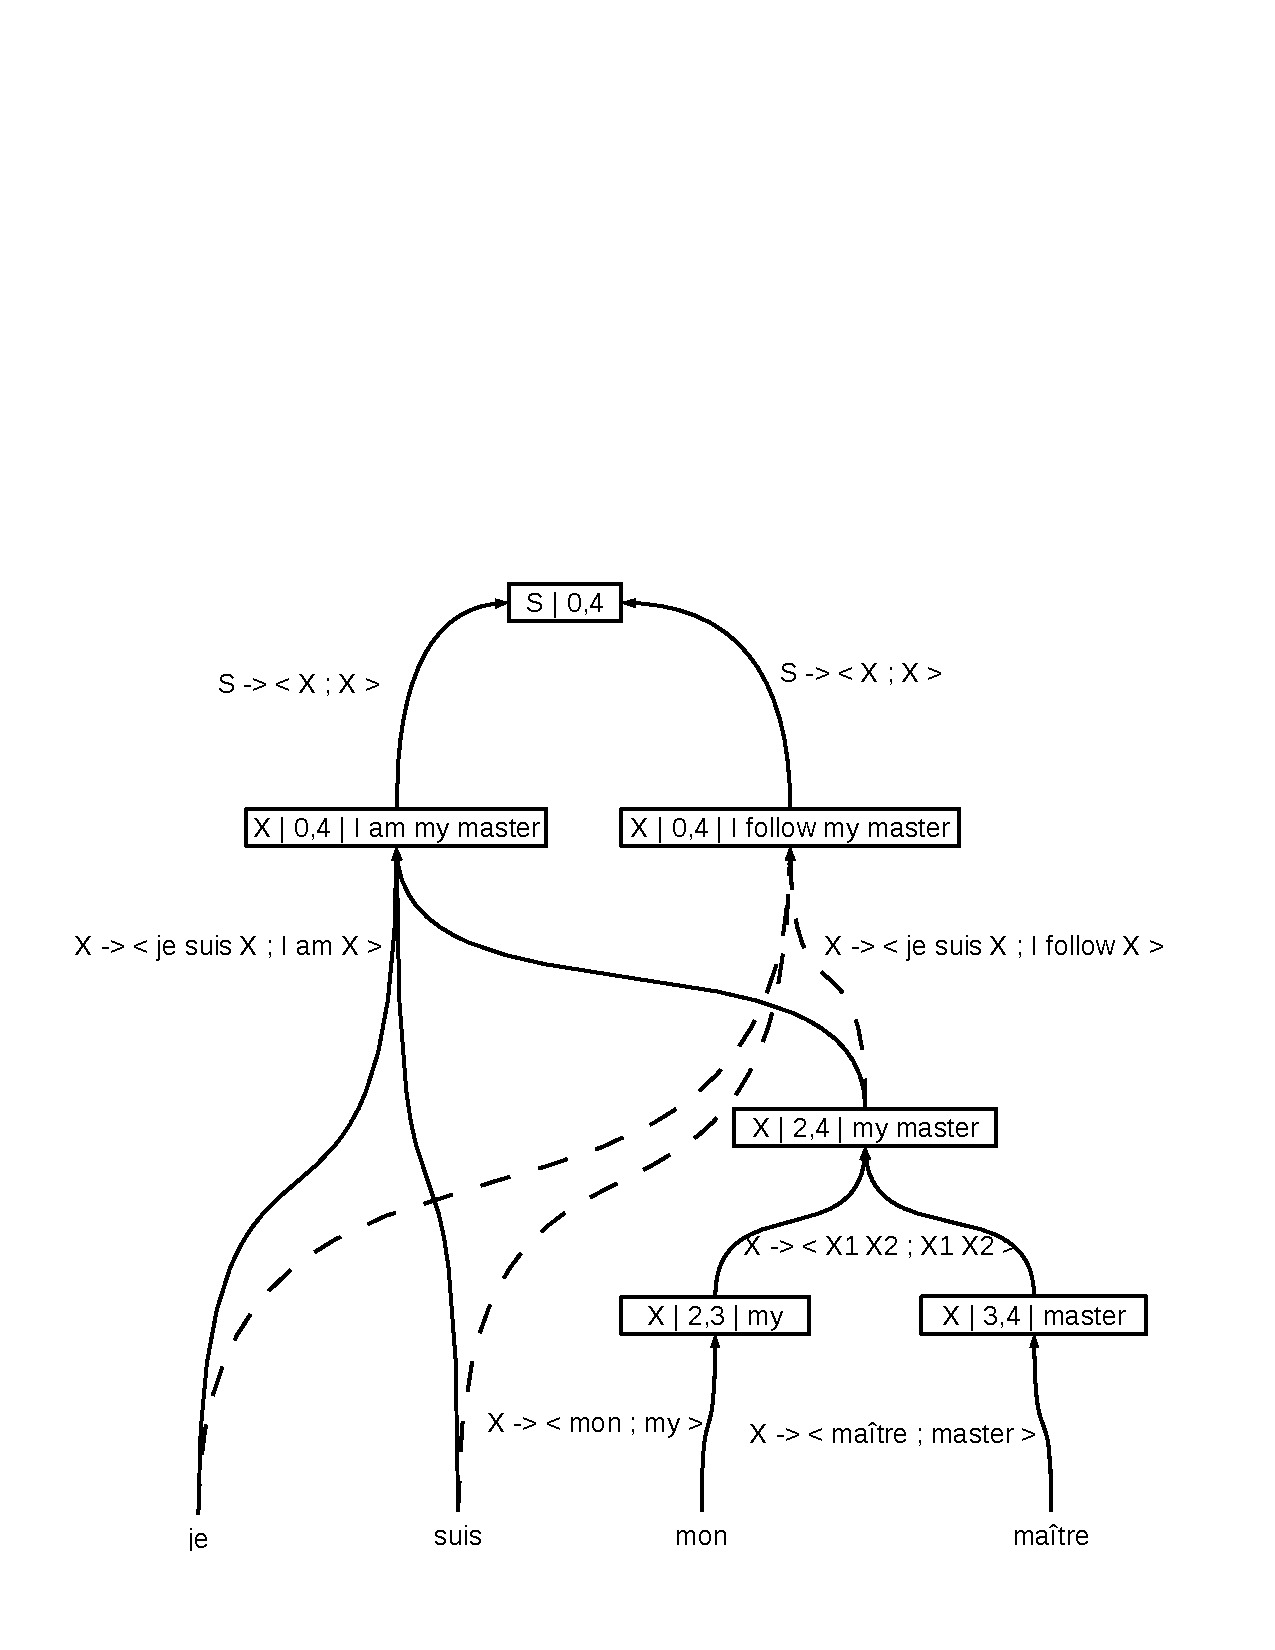
\includegraphics[width=\linewidth]{images/hypergraph-example}
%\end{center}
%\caption{A hypergraph showing two candidate translations of {\it Je suis mon ma\^{i}tre}.}
%\label{hypergraph-example-figure}
%\end{wrapfigure}    
%
Figure \ref{hypergraph-example-figure} shows an example of a hypergraph with
two candidate translations for the French sentence ``{\it Je suis mon
ma\^{i}tre}.'' Note that both translations --- ``I am my master'' and ``I
follow my master'' --- use the same derivation of ``my master'' as a phrasal
translation for the French {\it mon ma\^{i}tre}. Therefore, the hypergraph
maintains only one copy of this shared structure, saving space.

%The hypergraph is a representation of each of the choices
%made by the decoder during the decoding process:
%parsing with a SCFG is just choosing which production rules to use
%and in which order they should be applied.
%Each node of the hypergraph then represents a ``choice point'' that affects
%which candidate translation is evetually produced. In general, exponentially
%many derivations can be enumerated from the hypergraph by selecting different
%production rules at each choice point.

We focus on two data structures
used in the decoding process: first, each candidate translation has a {\em
derivation tree} describing how the decoder generated the candidate. Second,
there is a {\em hypergraph} that represents {\em all} the choices made by the
decoder when translating a single input sentence and shows us the relationships among all the various candidates.
%The visualization tools included with Joshua let the researcher inspect both
%of these data structures.


\section{Joshua's Visualization Tools}


\begin{figure}
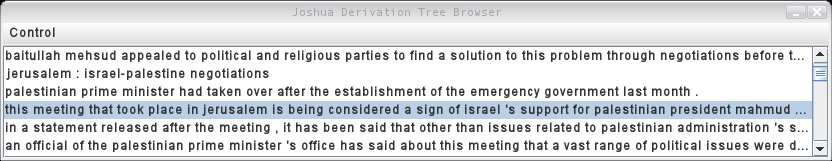
\includegraphics[width=.95\linewidth]{images/pick-window-2} 
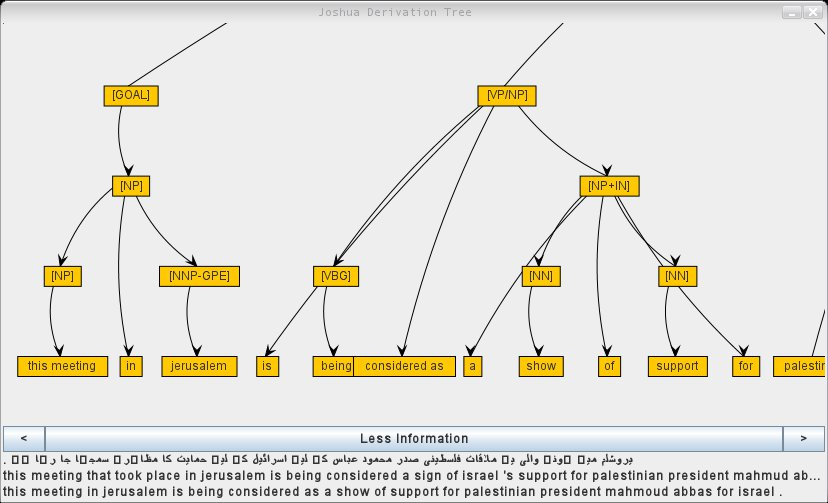
\includegraphics[width=\linewidth]{images/urdu-tree-window-2}
\caption{The Derivation Tree browser's sentence selection and tree-viewing windows.}
\label{derivation-figure}
\end{figure}




The visualization tools are included in the Joshua Decoder release.\footnote{\url{http://cs.jhu.edu/~ccb/joshua/}} They have
only one outside dependency: the Java Universal Network/Graph Framework\footnote{\url{http://jung.sourceforge.net/}} (JUNG), a toolkit for drawing graphs in Java,
which is available under the BSD License.

The derivation-tree viewer does not depend on the Joshua decoder. It can
visualize any derivation tree as long as the tree representation is identical
to Joshua's output. The hypergraph visualizer, on the other hand, depends
on the decoding process itself, and therefore on the Joshua decoder.

\subsection{Synchronous Derivation Trees}


The Joshua decoder includes an option to output text-based representations
of the target-side parse tree rather than the plain candidate translation.
These textual representations can also be annotated with the source-side
span of each nonterminal in the tree. 
(These outputs can be chosen by setting {\tt use\_tree\_nbest} and {\tt 
include\_align\_index} to true in the Joshua configuration
file.)
The core of the derivation-tree visualizer
 takes a string that represents an annotated parse tree and uses JUNG to draw
a graph representing the tree.

Using the source-side annotations, the visualizer also draws the 
parse tree for the input sentence. Since the grammar is synchronous, there is
a one-to-one correspondence between nonterminals in the source- and target-side
trees. Any differences in the tree structure arise from possible reordering
of the nonterminals.
The bottom of Figure \ref{derivation-figure} shows part of the derivation tree 
generated by Joshua's output of 
% ccb - I manually inserted some newlines to make this wrap properly. 
{\tt (ROOT\{0-24\} ([GOAL]\{0-23\} ([GOAL]\{0-6\} ([NP]\{0-6\} ([NP]\{4-6\} this meeting) in ([NNP-GPE]\{0-1\} jerusalem))) ([S]\{6-23\} ([VP/NP]\{14-22\} is 
 \\
 ([VBG]\{19-21\} being) considered as ([NP+IN]\{14-18\} a ([NN]\{17-18\} show) of ([NN]\{15-16\} support) for)) ([NP]\{6-14\} palestinian ([JJ-GPE-ite\textbackslash NP]
 \\
\{7-14\} president ([NP-PERSON]\{8-10\} mahmoud abbas) ([PP]\{10-14\} for 
 \\
 ([NNP-GPE]\{12-13\} israel)))) .)))}


The tree visualizer takes the following arguments:  a file containing source-side sentences (one per line), a file containing the parallel target-side reference translations, and then one or more files containing n-best translations of the source sentences.
Multiple n-best files can be specified in order to contrast different runs
of the decoder on the same test set. For example, Figure \ref{example-derivations} shows one
sentence from the 2009 NIST Urdu--English evaluation, decoded once under a 
Hiero-style grammar with only one nonterminal symbol X, as introduced in
\cite{Chiang2005}, and once under a
syntactically-motivated grammar with a richer nonterminal set as  presented in \cite{samt2006}.

\begin{figure}
\begin{center}
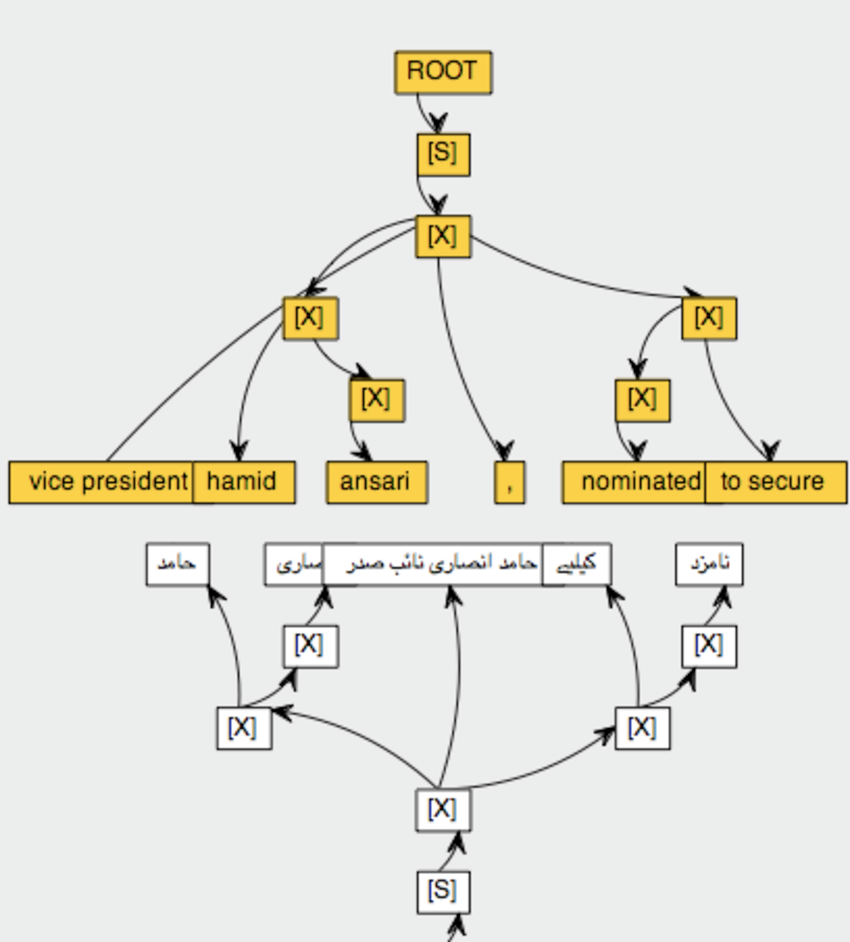
\includegraphics[height=2.75in]{images/hiero-tree}
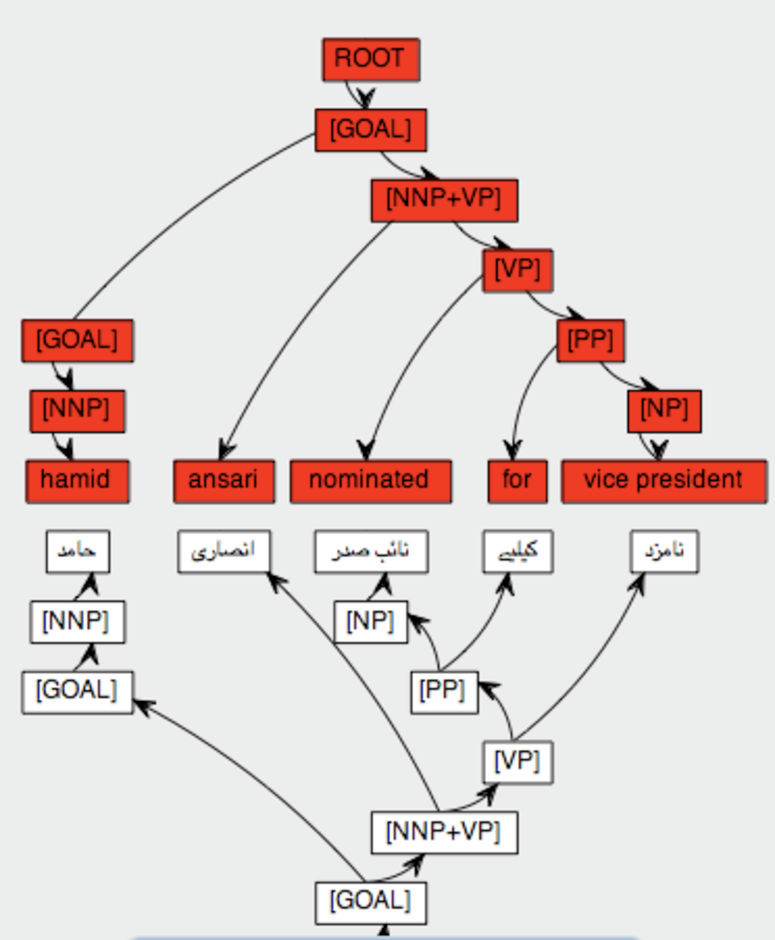
\includegraphics[height=2.75in]{images/samt-tree}
\end{center}
\caption{An example visualization of two derivation trees for SCFGs that use a Hiero-style grammar and a syntactically-motivated grammar.}\label{example-derivations}
\end{figure}

When the visualizer starts up, it creates two types of windows. First there is
a window listing all the reference translations.
This window is shown on the top of Figure \ref{derivation-figure}.
(This is the reason for the
reference translation file --- an earlier version of the program had the 
sentences listed by the source side, but this was less useful for users who
had no knowledge of the source language.) The second type of window displays
a derivation tree.

The browser creates one tree-displaying window 
(as seen on the bottom of Figure \ref{derivation-figure})
for every n-best file that is
passed as an argument. This allows the user to easily compare derivation trees
created by different grammars (these are saved in different n-best files,
since they're the result of different runs of the decoder). In a tree window,
the user can click and drag to inspect different parts of the tree and can use
the scroll wheel to zoom in and out.

There are two ways to change trees: clicking the sentence in
the list window or using the left- and right-arrow buttons in the tree windows.
In either case, all the tree windows are synchronized; that is, whenever the
user changes to a different sentence, all tree windows are updated to show
the derivation for that sentence. The tree views are anchored; for example, if
a user were zoomed in on the first target-side nonterminals of one tree, when
he changed to a new sentence and the new tree was displayed, its view would
start zoomed in on that same area of the new sentence's tree.

The tree view windows also have a button to give the user more information about the current tree.  This button shows the source sentence, the reference translation, and the text of the translation candidate.

\subsection{Hypergraphs}

\begin{figure}
%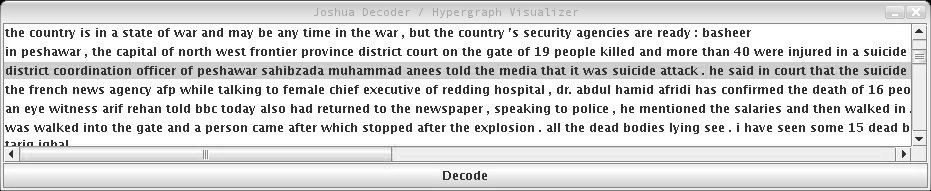
\includegraphics[width=.95\linewidth]{images/bw/hg-pick-window-2-bw}
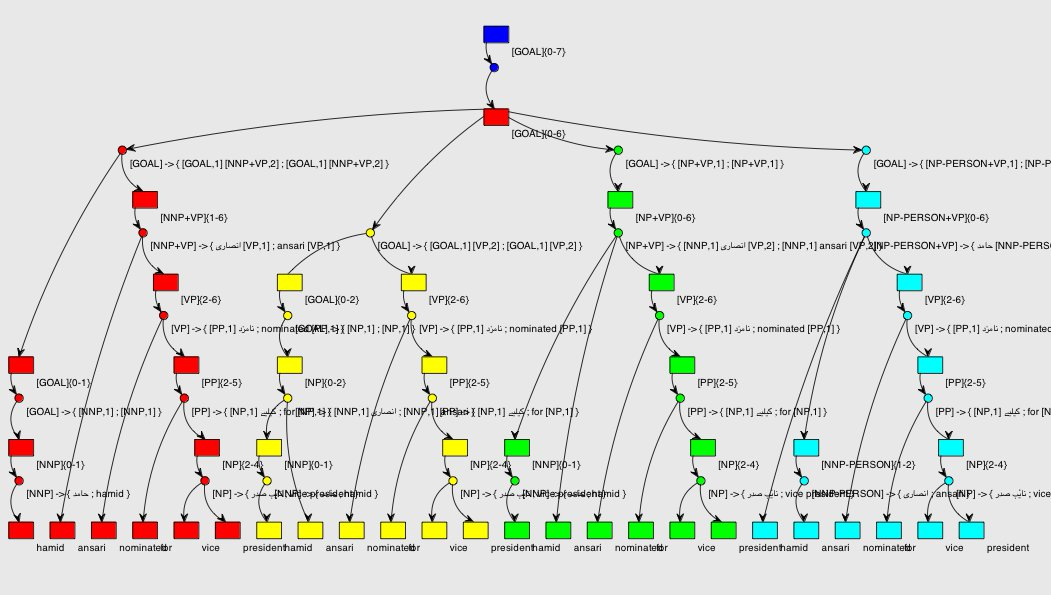
\includegraphics[width=\linewidth]{images/hamid-ansari-derivations-cropped}
\caption{The visualization window for the hypergraph browser.}
\label{hypergraph-screenshot}
\end{figure}


The derivation tree viewer is used after running the decoder to inspect its
ouput. Since the hypergraph is used during the decoding process and is
discarded afterwards, the hypergraph visualizer depends on the decoder itself.
Internally, it works by setting a flag to build the graph visualization 
on-the-fly as the decoder processes the input.

The command line arguments for the hypergraph visualizer are slightly
different from the derivation tree viewer. A reference translation
is used in the same way as in the derivation tree viewer --- it allows the user
to choose a sentence to translate based on the reference translation. Now
because the decoder translates source sentences on demand, the other two
arguments are a source-sentence file and a Joshua configuration file that
should be used for the decoding.

On startup, the hypergraph viewer presents a list of sentences to translate.
%This window is shown on the top of Figure \ref{hypergraph-screenshot}.
The reference translations are displayed instead of the source to make it easier for the user. The user selects a sentence from the list and presses the ``Decode'' button at the bottom. Internally, the hypergraph viewer chooses the associated source sentence and calls Joshua to decode the sentence using the supplied
configuration file.

As the hypergraph structure is constructed, the
hypergraph viewer uses JUNG to build a corresponding graph. At first glance,
the graph that is displayed looks very similar to a derivation tree. In fact,
it is a hypergraph representation of the one-best candidate for the source
sentence.
Recall that the nodes of the hypergraph represent nonterminals or terminals in
the derivation of a given source sentence, and the hyperedges represent
production rules that are applied at each step.
Each node of the hypergraph is a rectangular box in this visualization, and
each hyperedge is a small circle. There may be many possible hyperedges leading
from a particular node, each one representing a different rule that could
be applied to that node. When only one hyperedge is visualized at each node,
the resulting graph represents one candidate translation.

Using the hypergraph viewer, we can inspect the choices that the decoder made
at each point. When the user clicks on a node of the hypergraph, a list of all
hyperedges leading from that node is displayed on the left. If the user selects
a hyperedge from the list, the corresponding subtree is displayed in the graph.
A user can even select multiple rules, and all of the resulting subtrees are
displayed side-by-side.
%The bottom of
Figure \ref{hypergraph-screenshot} shows this hypergraph view.
% On the list, two rules are selected, and the two corresponding subtrees,
% showing two distinct derivations of the phrase ``he said''  are generated
%in distinct colors below their parent node.
We can see four subtrees giving possible derivations of the 
candidate translation
``hamid ansari nominated for vice president.''

\section{Other Visualization Tools}

This section describes two other visualization tools developed by other
researchers, and contrasts the goals of the various visualization systems and
how the goals are reflected in design choices.

\subsection{The Chinese Room}

The Chinese Room \cite{albrecht-hwa-marai:2009:EACL} is a collaborative translation interface. It uses visualization
techniques to allow a user who has no knowledge of the source-side language to
collaborate with an MT system to create good translations. This is different
from earlier approaches to collaborative MT where the user was often assumed to
 be a professional translator. 

%The most important difference between the Chinese Room and Joshua's
%visualization tools is that they are designed for different goals.
The Chinese
Room is designed to allow {\em translators} (even those with limited or no
knowledge of the source language) to produce good translations of the input
sentences. Joshua's visualization tools, on the other hand, are designed to
help {\em researchers} debug grammars and improve their translation models.
%Naturally, observing a user's interaction with the Chinese Room may lead to
%improvements in a translation model, but the user's goal is, in the end, to
%decode the input sentence given.
%So naturally there are differences in the two visualization schemes. 
The Chinese Room tries to give the user as much information as possible to
create a correct translation. This includes word alignments, glosses for
source words from a dictionary, source-side parse structure and so on. All
of this information would be useful for a translator.
%On the other hand, 
The current tools for Joshua are focused on improving
the grammars used in a translation model. We need comparatively less 
information to gain useful insight into this smaller domain. That is why we
have focused only on displaying the derivation trees and hypergraphs.
%We are interested in analyzing and correcting the mistakes that the decoder
%drew from the grammar, rather than helping a human to avoid those mistakes
%during the translation process.

\subsection{DerivTool}

DerivTool is a tool for interactively directing the decoding of a sentence
using a syntax-based MT model \cite{deneefe-knight-chan:2005:PosterDemo}. Users can choose which
rules to apply to a derivation at which time. In the end, the user ends up
building up a derivation tree for a particular candidate translation. DerivTool
is useful for analyzing grammars: a user can immediately tell when a needed
rule is missing (they can't continue their intended derivation) and can see
which rules are favored by the decoder at a particular point (since rules are
displayed in order of frequency).

%Since Joshua also visualizes derivation trees, we can consider DerivTool and
%Joshua as two tools that produce the same result (that is, they are visualizing
%the same data structure in the end). The main difference is whether the
% process is interactive or not. Both interactivity and batch-mode usage
% have their advantages.

Joshua's tools and DerivTool both produce derivation trees. The difference is that DerivTool is interactive and Joshua is not.
The main advantage of working in batch mode is that it is faster than building
up a derivation tree manually step-by-step. We run the decoder seperately,
letting it make the translation decisions. Afterwards,
the user can evaluate the quality of the trees produced. The Joshua
visualization tool can produce many derivation trees all at once (it reads
in a file containing the n-best derivations for each sentence of a test set).
This makes it easy to compare the different decisions that were possible at
decoding time without the user having to manually make the decisions himself.

\section{How Joshua's Visualization Tools Help}
\begin{figure}
\begin{center}
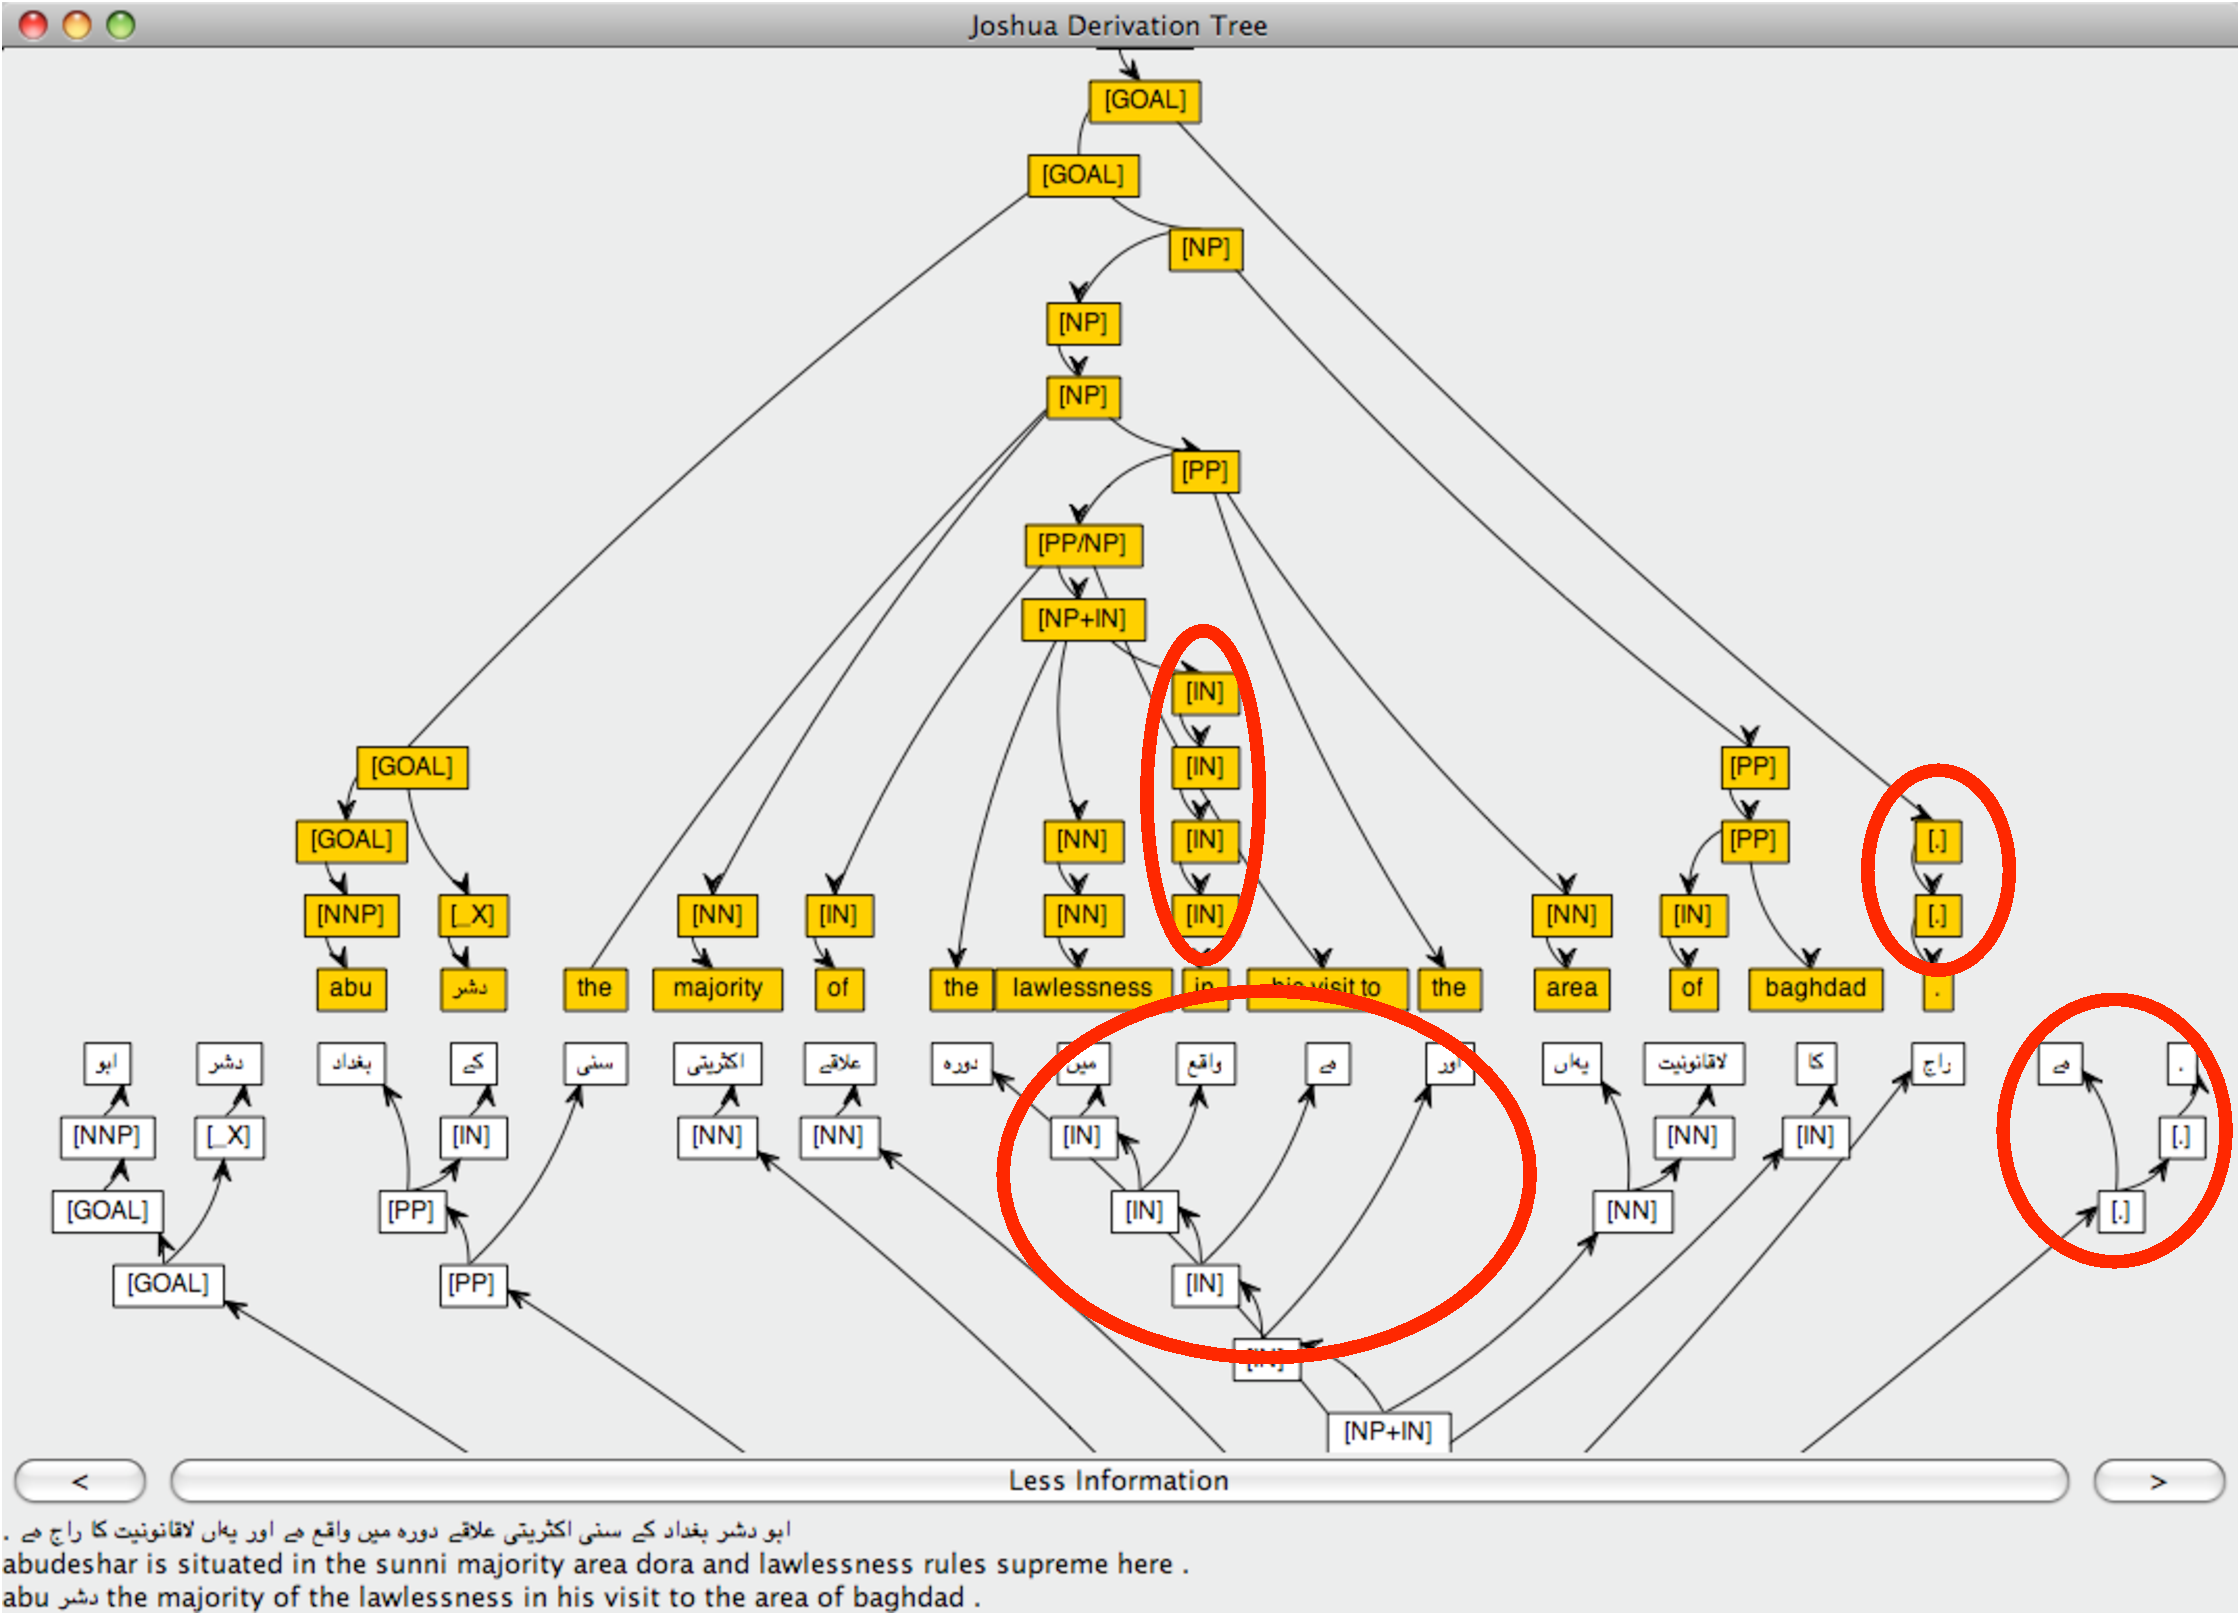
\includegraphics[height=3in]{images/terminals-being-eaten-highlights}
\end{center}
\caption{An example of bad production rules that parse pieces of the source
sentence without producing any target-side output.}
\label{terminals-being-eaten}
\end{figure}



By visualizing derivation trees for different candidate translations, we
can find problems with the SCFGs that underly translations.
For example, we used the visualization tool to inspect derivation trees that were produced on the 2009 NIST
Urdu--English test set,
and noticed that many rules consumed part of the input sentence without producing any
output.  These rules were used often in the top candidates, but brought
down the translation quality. Having discovered that, we manually removed %rules of the form
%$$\textrm{X} \to \langle \gamma, \alpha, \sim, w\rangle$$
%where $\alpha$ is a string of nonterminals with no target-side terminal
%symbols. This helped improve the translation quality.
where the target side contained no terminal symbols.
This helped improve the translation quality.
In Figure \ref{terminals-being-eaten}, we can see rules of the form
$\textrm{[IN]} \to \langle \textrm{[IN]}\gamma,\textrm{[IN]}\rangle$ and
$\textrm{[.]} \to \langle \textrm{[.]}\gamma, \textrm{[.]}\rangle$ being
applied.

Pruning grammars of systematically bad production rules is a good way to
improve translation quality, and manual inspection of the output to see which
grammar rules have been used, and which ones correlate with low translation
quality, is an effective way to prune.
The derivation tree visualizer helps researchers too notice patterns in rule
application among different candidate translations.

Visualizing hypergraphs lets the researcher inspect the decisions that the
decoder made when choosing among different rules that could be applied at some
point in a derivation. This could be useful, for example, in determining if
a particular type of rule is being systematically overweighted or underweighted,

Visualizing the data structures involved in MT decoding allows the researcher
to determine empirical rules for improving the grammars involved.

%First, we can tell at a glance whether the parse tree seems ``reasonable.''
%That is, the intuition behind the SCFG formalism suggests that parse trees
%should have the right shape on both the source and target side. A single
%phrase should be the output of a single subtree; two phrases should be
%combined in a particular way, and so on. A grammar that produces excessively
%branching trees, for example, can be noticed immediately by looking at the
%tree itself.

%Secondly, we can do a more fine-grained analysis of the candidate. Maybe some
%parts of the translation look reasonable, but others are way off. By examining
%the parse tree, we can tell what rules of the grammar give rise to bad
%translations by seeing which subtrees correspond to the bad translation.
%
%By examining candidate translations with similar errors, we can see what kinds
%of grammars correspond to good translations and what kinds of grammars cause
%errors.

%Visualizing the hypergraph gives us another useful perspective on the decoding
%process. Before, we were comparing the parse trees of individual candidates.
%This let us get a sense of which rules of the SCFG correspond to good
%translations and which ones do not. But by visualizing the hypergraph, we
%can see which rules are competing with each other during the decoding process
%itself.
%



\section{Future Work}

There are still many improvements that should be made to these visualization
tools. %The first is that
We would like to be able to show the terminal alignments
that are induced by a particular derivation. But that requires more information
than is currently given by the Joshua decoder.
It only annotates nonterminals with
source-side spans.
As an example, consider the French phrase {\it l'objectif de $X$ est de}
 which corresponds to the English phrase {\it the goal of $X$ is to}. We know
 that those two phrases have corresponding spans, and that the two $X$ symbols
 also correspond. But despite this, we don't have word-level alignment
information: we don't know if {\it l'objectif de} corresponds to {\it the goal
of} or to {\it is to}. Such fine-grained information would be useful for
visualizing reordering in MT models.

Another improvement that we think would greatly increase the utility of these
visualization tools for research is to add support for exporting the displayed
trees as files. It would be nice to be able to  save an interesting tree in PDF format so that it could be easily embedded in a research paper.

There are other parts of the Joshua pipeline that might benefit
from visualization. During rule extraction, SCFG rules are automatically
generated given an aligned parallel corpus. Being able to visually inspect
both the aligner output and the results of the rule extraction on an individual
phrase could provide some insight into this process.
The decoder works by CKY
parsing, so it would be advantageous for researchers to be able to view the
parse chart that is produced --- which constituents are generates where, what
their associated weights are, which ones have been pruned, and so on. This
 would help to determine if translation errors are caused by search errors
 or something else.

%As noted above, the derivation-tree viewer is static. It reads in a
%representation of a parse tree and renders it. It would be easier for the user
%to interpret a particular tree if the derivation itself were presented as an
%animation. The user could immediately see the results of a single rule being
%applied, as well as the effect of any re-ordering on the parallel parse tree.


\section*{Acknowledgments}
This research was supported in part by the EuroMatrixPlus project funded by
the European Commission under the Seventh Framework Programme, and by the US National Science Foundation under grant IIS-0713448.  The views and findings are the authors' alone. 

\bibliography{visualization}
\end{document}
